\chapter{Модел физике} \label{Collision}


Прво се са сензора детектује ново убрзање које делује на уређај (гравитационо + убрзање уређаја) и оно се филтрира да би се спречило превелике осцилације у убрзању, ако сензор нешто погрешно прочита. Даље филтрирано убрзање као и време кад је детектовано се прослеђују моделу са листом фигура и лоптом (позиција, полупречник). Ово је опис система до "предаје" управљања лопте класи \emph{CollisionModel}.
\\ \indent
Даље се убрзање скалира (множи са одговарајућим коефицијентом из подешавања апликације) што омогућава да лопта пуно брже реагује на промене убрзања уређаја.
Даље, лопта у сваком тренутку има вектор кретања брзине по све три осе $v_x, v_y, v_z$. Да би се израчунале нове брзине $v_x, v_y$ потребно је "потпуно" убрзање (сила) која делује на лопту. "Потпуно" убрзање се рачуна тако што се скалирано убрзање потом дода на трење (боље речено одузме). Трење се рачуна као убрзање по $z$ оси скалирано са коефицијентом трења добијеним из подешавања апликације, али тако да има знак супротан од брзине. Овај модел трења је реалистичан јер трење и у стварности је $\mu N$, где је $N$ нормална сила (на уређају је убрзање у суштини та нормална сила). Потом се нова брзина рачуна
$$v_i=v_{previousi} + a_{full}  \Delta T, i \in \{x, y\}$$
При чему је $a_{full}$ "потпуно" убрзање, $v_{previousi}$ претходна брзина лопте, а $v_i$ нова и $\Delta T$  разлика између времена претходне детекције сензора и тренутне детекције (који се обрађује). Ако је брзина променила смер по некој од оса и трење је утицало на то, брзина по тој оси постаје 0.
\\ \indent
Сад се рачунају потенцијалне нове позиције лопте по формули:
$$i = i_{old} + v_i \Delta T, i\in{x, y}$$
Где је $i$ нова координата центра лопте по одговарајућој оси, а $i_{old}$ стара координата. Потом се рачунају судари са свим фигурама на екрану И за оне фигуре са којима се сударила рачуна се како утичу на промену брзине. Све те фигуре утичу на промену брзине.  Постоје два типа фигура.
\\ \indent
\begin{figure}[htb!]
\begin{center}
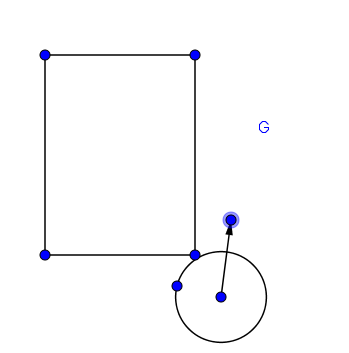
\includegraphics[scale=.5]{pictures/physics/ballRectDown}
\caption{Судар лопте и правоугаоника кад се лопта креће нагоре}\label{fig:ballRectDown}
\end{center}
\end{figure}
\begin{figure}[htb!]
\begin{center}
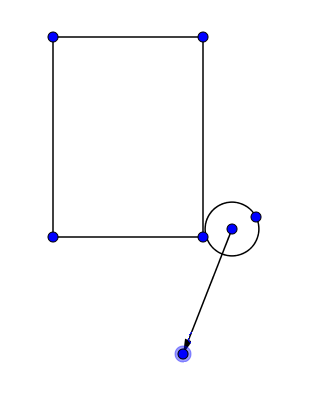
\includegraphics[scale=.5]{pictures/physics/ballRectUp}
\caption{Судар лопте и правоугаоника кад се лопта креће надоле}\label{fig:ballRectUp}
\end{center}
\end{figure}

Први су класичне препреке од које лопта одбија. Могу бити правоугаоне (квадрасте) или кружне (лоптасте).
За правоугаонке је коришћен упрошћен модел, где су странице правоугаоника паралелне осама.
Промена брзине рачуна тако да под оним углом којим је ушла мора да се и одбије (за случај кад удара само страницу правоугаоника, без ћошка).То је одрађено простом провером гледа се у коју страницу удари и онда ако је ударила у страницу чија је оса паралелна рецимо оси $x$ онда се мења брзина $y$ (враћа се негативна вредност по тој оси). Аналогно и за осу $y$.  Док кад удари ћошак врши се промена брзине по оси као у случајевима да није ћошак, али само под условом да се "приближава" тој ивици. Кад се каже приближава, мисли се у случају кад рецимо лопта прилази са доњој страници правоугаоника са доње стране, онда ће се "одбити" по $y$ оси (слика \ref{fig:ballRectDown}). Али рецимо у случају кад би прилазила са горње стране не би се одбила по $y$ оси (слика \ref{fig:ballRectUp}).   Ово спречава да се лопта "заглави" на ћошку, а и даје релативно реалистичан судар. Кад се ради са правоугаоницима којима странице нису паралелне осама, проблем се сведе на претходни. Извршимо просту ротацију читавог координатног система (уједно и брзине лопте) за угао $-\alpha$ при чему је $\alpha$ угао под којим се налази правоугаоник у односу на $x$ осу. Ротација се врши множењем сваке координате коју смо користили у старом систему ротационом матрицом \footnote{\url{http://mathworld.wolfram.com/RotationMatrix.html}}. Тако да је нови проблем сведен на већ решен. Проблем се реши као у претходном случају и онда се промена брзине само врати у почетни систем ротацијом промена брзине за $\alpha$. Пошто ротација захтева рачунање $\sin$ и $\cos$ коришћена је оптимизацје по којој су они израчунати унапред (кад се учитава полигон) и онда нема губитка времна при њиховом евалуирању.
\\ \indent
За кружне препреке тражена брзина је :
$$v_{new} = v_i - 2 \frac{\langle v_{old}, c_1 - c_2 \rangle (c_1 - c_2)}{||c_1-c_2 ||^2 }$$
При чему су $c_1$ стара координата центра лопте (пре потенцијалног померања), $c_2$ координата центра препреке са којом се лопта судара, $v_{old}$ брзина лопте као и $v_{new}$ брзина која треба да се добије. При чему је $|| nesto||$ ознака за дужину вектора, док је $\langle n_1, n_2 \rangle$ ознака за скаларни производ два вектора $nesto_1, nesto_2$. Промена брзине се рачуна:
$$v_{change} = \frac{v_{new} - v_{old}}{2}$$
Овај начин рачунања избегава било какво коришћење тригонометрије и због тога је брз.
\\ \
Друга врста препрека су рупе.
Има их три типа, али у суштини се све три понашају на исти начин.
Промена брзине се рачуна по формули:
$$v_{change} =  \frac{(c_2 - c_1) \cdot GRAVITY\_CON}{|| c_2-c_1||^2}$$
Овде су $c_2$ нова координата лопте, $c_1$ координата препреке. Док је $GRAVITY\_CON$ константа којом се лопта привлачи.
\\ \indent
Након што се израчунају промене брзине за све сударе у том тренутку лопте, оне се множе са 2 и све се сабирају. Након тога ако нема промене брзине по $x$ координати или је лопти промењена брзина под утицајем рупа лопта може да се помери на новоизрачунату координату по тој оси. Иначе по $x$ оси не може. Аналогно је и за $y$ осу. На крају брзина се мења додавањем збира промена брзине по тој оси на брзину генерисану након рачунања "потпуног" убрзања. Oод условом да је брзина промене различита од 0 или под условом да се лопта "сударила" са рупом претходно израчуната брзина губи одређен проценат који је подешен у подешавањима апликације.


